\documentclass[11pt,a4paper]{article}
\usepackage[T1]{fontenc}
\usepackage{lmodern}
\usepackage[margin=2.2cm]{geometry}
\usepackage{amsmath,amssymb}
\usepackage{booktabs,tabularx,array}
\usepackage{graphicx}
\usepackage{float}
\usepackage{xcolor}
\usepackage{tikz}
\usetikzlibrary{arrows.meta,positioning}
\usepackage[hidelinks]{hyperref}
\def\sectionautorefname{Section}\def\subsectionautorefname{Section}

\definecolor{navy}{HTML}{1F3A5F}
\definecolor{soft}{HTML}{EEF3FA}
\definecolor{todo}{HTML}{FDF1E9}
\definecolor{todoline}{HTML}{EB6834}
\newcommand{\code}[1]{\texttt{\small #1}}
\newcommand{\bs}{\textbackslash}
% A box the author fills in: the course does not allow LLM-written analysis or conclusions.
\newcommand{\authorbox}[2]{\par\smallskip\noindent\fcolorbox{todoline}{todo}{\parbox{\dimexpr\linewidth-2\fboxsep-2\fboxrule}{%
  \small\textbf{To be written by the author --- #1}\par\smallskip #2}}\par\smallskip}

% generated by make_figures.py
\newcommand{\bertRtwoAfour}{0.8358}
\newcommand{\bertRtwoAone}{0.8359}
\newcommand{\bertRtwoAthree}{0.8341}
\newcommand{\bertRtwoAtwo}{0.8245}
\newcommand{\bertRzeroAfour}{0.8269}
\newcommand{\bertRzeroAone}{0.8286}
\newcommand{\bertRzeroAthree}{0.8255}
\newcommand{\bertRzeroAtwo}{0.8170}
\newcommand{\contamPone}{226}
\newcommand{\contamPtwo}{26}
\newcommand{\fairRoneAfour}{11.25}
\newcommand{\fairRoneAone}{11.82}
\newcommand{\fairRoneAthree}{12.42}
\newcommand{\fairRoneAtwo}{22.31}
\newcommand{\fairRtwoAfour}{8.26}
\newcommand{\fairRtwoAone}{8.37}
\newcommand{\fairRtwoAthree}{8.98}
\newcommand{\fairRtwoAtwo}{13.12}
\newcommand{\fairRzeroAfour}{13.32}
\newcommand{\fairRzeroAone}{12.93}
\newcommand{\fairRzeroAthree}{13.89}
\newcommand{\fairRzeroAtwo}{25.26}
\newcommand{\fairgainRoneAfour}{15.5}
\newcommand{\fairgainRoneAone}{8.6}
\newcommand{\fairgainRoneAthree}{10.6}
\newcommand{\fairgainRoneAtwo}{11.7}
\newcommand{\fairkept}{1,990}
\newcommand{\fairtokens}{2.04M}
\newcommand{\fairtotal}{3,764}
\newcommand{\leakRtwoAfour}{7.17}
\newcommand{\leakRtwoAone}{7.23}
\newcommand{\leakRtwoAthree}{7.76}
\newcommand{\leakRtwoAtwo}{11.75}
\newcommand{\leakRzeroAfour}{18.75}
\newcommand{\leakRzeroAone}{17.49}
\newcommand{\leakRzeroAthree}{19.46}
\newcommand{\leakRzeroAtwo}{38.32}
\newcommand{\nearduppairs}{1,688,774}
\newcommand{\newtraintokens}{1.006B}
\newcommand{\newvaltokens}{4.10M}
\newcommand{\oldtraintokens}{187.5M}
\newcommand{\oldvaltokens}{4.96M}
\newcommand{\origpplAfour}{11.53}
\newcommand{\origpplAone}{11.36}
\newcommand{\origpplAthree}{12.11}
\newcommand{\origpplAtwo}{21.79}
\newcommand{\scavailable}{248M}
\newcommand{\speedupAfour}{5.1}
\newcommand{\speedupAone}{3.6}
\newcommand{\speedupAthree}{2.6}
\newcommand{\speedupAtwo}{3.3}
\newcommand{\totavailable}{2,668,667}
\newcommand{\totdocsread}{3,480,220}
\newcommand{\totexactdup}{106,717}
\newcommand{\totfewletters}{29,393}
\newcommand{\totneardup}{204,246}
\newcommand{\totreplacementchar}{528}
\newcommand{\totstutter}{90,856}
\newcommand{\totstutterrepaired}{125,397}
\newcommand{\totstutterwords}{2.34M}
\newcommand{\tottooshort}{379,813}
\newcommand{\tribdeva}{22,774}
\newcommand{\tribdevapct}{12.8}
\newcommand{\tribnonascii}{841}
\newcommand{\valleakdropped}{764}

\makeatletter\newcommand{\tabinput}[1]{\@@input #1 }\makeatother % expandable \input inside tabulars

\title{\textbf{CS-781 Capstone, Phase 1: Legal Language Model Pre-training}\\[2pt]
\large Four architectures, a corpus audit, a cleaned 1B-token corpus, and retraining}
\author{Manish Kumar (251330604)\\ CS-781, IIT Kanpur}
\date{October 2026}

\begin{document}
\maketitle

\begin{abstract}
\noindent We train four substantially different legal language models (50--300M parameters) from scratch on
the Phase-1 Indian legal corpus: a decoder-only GPT (A1), an encoder--decoder (A2), a prefix-LM with ALiBi
(A3) and an efficient decoder with RoPE, grouped-query and sliding-window attention (A4).  The first runs use
the starter budget of about 200M tokens.  An audit of that corpus found validation documents copied in the
training split, duplicates, OCR word stutter and encoding residue, so we built a second data pipeline:
whole-file sampling, character and markup normalisation, stutter repair, quality filters, exact and MinHash
near-duplicate removal, a measured token budget, and a validation split that shares no text with either
training corpus.  We also made training \speedupAfour$\times$ faster for A4 (\speedupAone$\times$ for A1) with
the same effective batch.  On a validation set that neither corpus contains, retraining on the cleaned
corpus at the same 200M-token budget lowers perplexity for every architecture (A4: \fairRzeroAfour{} $\to$
\fairRoneAfour), and continuing to 1B tokens lowers it further (A4: \fairRtwoAfour; A1: \fairRtwoAone).
Dev BERTScore F1 rises from \bertRzeroAfour{} to \bertRtwoAfour{} for A4.  All numbers in this report are
generated from the run outputs by \code{p1/report/make\_figures.py}.
\end{abstract}

\tableofcontents
\newpage

% =====================================================================
\section{Introduction}
Phase~1 asks for a legal language model trained from scratch on the provided corpus of Acts, High Court,
Supreme Court and Tribunal documents, which continues a 512-word legal prompt with 128 words.  Submissions
are scored with BERTScore F1 (primary), ROUGE-L F1 and BLEU-4.  The rules fix the model size (50M--300M
parameters), forbid pretrained weights and external corpora, require at least four substantially
different architectures, and ask that training stay practical on free Colab/Kaggle-class hardware.  The
Phase-1 models are also the starting point for Phases~2--7, so their usefulness as encoders matters as much
as their generation scores.

This report documents the whole Phase-1 work in the order it happened:
\begin{enumerate}
  \item the starter-notebook baseline (\autoref{sec:baseline});
  \item a controlled comparison of four architectures on one data pipeline (\autoref{sec:arch}, \autoref{sec:setup} and \autoref{sec:res-orig});
  \item an audit of that data, which found nine problems (\autoref{sec:audit});
  \item a cleaned corpus that addresses them (\autoref{sec:cleaning} and \autoref{sec:res-clean});
  \item faster training without changing the optimisation (\autoref{sec:throughput} and \autoref{sec:res-tput});
  \item retraining all four architectures on the cleaned corpus, evaluated on three validation sets
        (\autoref{sec:retrain}, \autoref{sec:res-retrain} and \autoref{sec:res-eval}), and checks of test-set contamination (\autoref{sec:res-contam}).
\end{enumerate}

% =====================================================================
\section{Data and tokenizer}\label{sec:data}
\subsection{The Phase-1 corpus}
The corpus has four training sources (\code{train\_acts.json} 0.7\,GB, \code{train\_supreme\_court.json}
1.3\,GB, \code{train\_tribunals.json} 6.5\,GB, \code{train\_high\_courts.json} 10.7\,GB; more than 4.5B
tokens in total) and a test file of 1{,}000 prompts.  No validation split is provided.

\subsection{First data pipeline}\label{sec:firstpipe}
The first pipeline (\code{legal\_lm/data/corpus.py}) streams each file with \code{ijson}, keeps a document
with probability 0.5, collapses whitespace, drops documents under 50 words, sends 1\% of the kept documents
to validation, and stops reading a source once its share of the budget is filled.  The mixing ratios are
Acts 10\%, Supreme Court 30\%, High Courts 35\%, Tribunals 25\%; the budget is counted in words with an
assumed 1.35 tokens per word.  \autoref{tab:corpus-old} shows what it produced: \oldtraintokens{} training
tokens and \oldvaltokens{} validation tokens.

\begin{table}[H]\centering\small
\caption{First corpus (head-of-file sample). Tokens/word is measured with the legal BPE.}\label{tab:corpus-old}
\begin{tabular}{lrrrrr}\toprule
Source & Docs read & Train docs & Train words & Train tokens & Tokens/word\\\midrule
\tabinput{tables/corpus_old.tex}
\bottomrule\end{tabular}\end{table}

\subsection{Tokenizer}
A byte-level BPE \cite{sennrich2016bpe} with a 32{,}000-token vocabulary is trained on 100{,}000 documents of
the training split (\code{scripts/02\_train\_tokenizer.py}).  Byte-level BPE never produces unknown tokens
(Devanagari names, section symbols and OCR debris all encode), and a legal vocabulary keeps frequent words
such as \emph{respondent} or \emph{Section} as single tokens: the measured fertility is 1.21--1.46 tokens
per word depending on the source (\autoref{tab:clean-select}), so a 512-word prompt fits in roughly 700
tokens of a 1{,}024-token context.  The same tokenizer is used by every model in this report, and by
Phases~2--7.

% =====================================================================
\section{Methods}
\subsection{Starter baseline (B0)}\label{sec:baseline}
The course notebook (\code{p1/p1\_start.ipynb}) trains a randomly initialised GPT-2 model with the GPT-2
tokenizer: 8 layers, 8 heads, width 560, context 2{,}048, 59.5M parameters, 200M training and 5M
validation tokens, one epoch, AdamW at $3\times10^{-4}$ with cosine decay, about 0.63 GPU-hours at
88k tokens/s.  It reached a validation loss of 2.733 (perplexity 15.38).  Because the GPT-2 tokenizer
splits legal text differently, its per-token perplexity is not comparable with the legal-BPE models
below; it is kept as the starting reference only.

\subsection{Four architectures}\label{sec:arch}
All four models share the tokenizer, data, token budget, schedule and evaluation, so that only the
architecture changes (\autoref{tab:arch}).  Embeddings are tied with the output layer in every model.

\begin{table}[H]\centering\small
\caption{The four Phase-1 architectures (32k vocabulary, context 1{,}024).}\label{tab:arch}
\begin{tabularx}{\linewidth}{lXr}\toprule
ID & Design & Params\\\midrule
A1 GPT & Decoder-only \cite{radford2019gpt2}: learned absolute positions, pre-LayerNorm, GELU MLP, full causal
multi-head attention. 8 layers, $d=768$, 12 heads, $d_\text{ff}=3072$. & 82.1M\\
A2 enc-dec & Encoder--decoder \cite{vaswani2017attention}: bidirectional prompt encoder (6 layers) and causal
decoder with cross-attention (6 layers), sinusoidal positions, ReLU MLP. $d=640$, 10 heads,
$d_\text{ff}=2560$. Trained on a random split point: the encoder reads a prefix of $L/4$ to $L-64$
tokens, the decoder predicts the rest. & 89.4M\\
A3 prefix-LM & One stack whose mask makes the prompt bidirectional and the continuation causal
(UniLM/GLM style \cite{raffel2020t5}), ALiBi relative positions \cite{press2022alibi}, no position embeddings.
8 layers, $d=768$, 12 heads. With probability 0.5 an example is fully causal; otherwise a prefix of
64 to $0.75L$ tokens is read bidirectionally and only the rest is supervised. & 81.3M\\
A4 efficient & Decoder with RoPE \cite{su2021roformer}, RMSNorm \cite{zhang2019rmsnorm}, SwiGLU MLP
\cite{shazeer2020glu} ($d_\text{ff}=2048$), grouped-query attention \cite{ainslie2023gqa} (12 query heads,
4 key/value heads), sliding-window attention of 256 tokens \cite{beltagy2020longformer} with a global layer
every third layer. 10 layers, $d=768$. & 87.5M\\
\bottomrule\end{tabularx}\end{table}

\subsection{Training and evaluation setup}\label{sec:setup}
\begin{itemize}
  \item \textbf{Optimisation.} AdamW \cite{loshchilov2019adamw} ($\beta=(0.9,0.95)$, weight decay 0.1 on
  matrices only), peak learning rate $6\times10^{-4}$, 200 linear warm-up steps, cosine decay to
  $6\times10^{-5}$, gradient clipping at 1.0, bf16 autocast, no dropout.
  \item \textbf{Batch.} 8 sequences $\times$ 8 accumulation steps $\times$ 1{,}024 tokens = 65{,}536 tokens per
  optimizer step; 3{,}000 steps = 196.6M tokens, about one pass over the first corpus.  Training windows are
  sampled at random positions of a memory-mapped \code{uint16} token file.
  \item \textbf{Validation and checkpoint selection.} Every 250 steps, 40 fixed batches of 1{,}025-token
  windows are scored: the first 768 tokens are context and the loss is the mean over the next 257 tokens,
  mirroring the task (continue a prompt).  The checkpoint with the lowest validation loss is kept
  (\code{best.pt}); \code{last.pt} also stores the optimizer for resuming.
  \item \textbf{Generation.} Temperature 0.8, top-$k$ 50, top-$p$ 0.95 \cite{holtzman2020curious}, repetition
  penalty 1.1 \cite{keskar2019ctrl} over the last 256 tokens, end-of-text banned until 128 words are produced.
  \item \textbf{Generation metrics.} 200 local dev prompts (512 words + the true next 128 words) are cut from
  held-out documents; BERTScore F1 \cite{zhang2020bertscore}, ROUGE-L F1 \cite{lin2004rouge} and BLEU-4
  \cite{papineni2002bleu} are computed as on Codabench (\code{scripts/06\_evaluate.py}).
\end{itemize}

\subsection{Corpus audit}\label{sec:audit}
After the first runs we audited the training and validation splits (\code{scripts/11\_audit\_corpus.py}).
\autoref{tab:audit} lists the problems, labelled A--I; each is addressed by one or more of the methods M1--M10
in \autoref{sec:cleaning} (mapping in \autoref{tab:map}).

\begin{table}[H]\centering\small
\caption{Problems found in the first corpus.}\label{tab:audit}
\begin{tabularx}{\linewidth}{clX}\toprule
& Problem & Evidence\\\midrule
A & Under-trained base model & \oldtraintokens{} of $>$4.5B available tokens; about 20 tokens per parameter
\cite{hoffmann2022chinchilla} would be $\approx$1.7B for an 87M model; validation loss still falling at the end
of the schedule (\autoref{fig:val-orig}).\\
B & Validation leaks into train & 29 validation documents are exact copies of training documents; at least
52 of 500 sampled validation documents share more than half their word 13-grams with a 30k-document training
sample.\\
C & No deduplication & 1{,}090 exact duplicate training documents (0.7\%); 1{,}176 extra copies of the same
first 300 characters; one Bombay HC form header occurs 28 times.\\
D & OCR word stutter & 566 documents with five or more tripled words (``Parekh Parekh Parekh Petitioner
Petitioner Petitioner''), about 2.4M words.\\
E & Encoding / markup noise & About 70 documents with the replacement character U+FFFD, RTF control words
(\code{\bs par \bs pard \bs tab}), 513 Acts documents with runs of 20+ dots or dashes.\\
F & Short template orders & 32\% of High Court documents have fewer than 200 words (median 291 words).\\
G & Token budget missed & Budget estimated at 1.35 tokens/word; measured 1.21--1.32, so training got
\oldtraintokens{} instead of 200M tokens.\\
H & Head-of-file sampling & Each file is read from its first record until the budget fills, so documents
later in a file are never seen.\\
I & Long-range downstream labels & (Phase~2) party roles are declared in the header and must be resolved
thousands of tokens later; recorded here because it motivates longer context.\\
\bottomrule\end{tabularx}\end{table}

\subsection{Cleaned corpus}\label{sec:cleaning}
The second pipeline is \code{legal\_lm/data/clean.py}, enabled by \code{configs/clean.yaml}
(\autoref{tab:cleancfg}).  \autoref{fig:pipeline} shows the order of the steps.

\begin{figure}[H]\centering
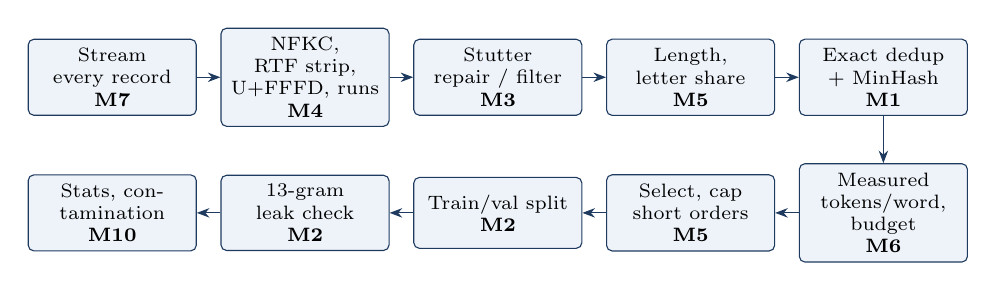
\begin{tikzpicture}[node distance=3mm, box/.style={draw=navy,rounded corners=2pt,fill=soft,align=center,
  font=\scriptsize,minimum height=9mm,text width=19mm}, arr/.style={-{Stealth[length=1.6mm]},navy}]
  \node[box] (a) {Stream every record\\\textbf{M7}};
  \node[box,right=of a] (b) {NFKC, RTF strip, U+FFFD, runs\\\textbf{M4}};
  \node[box,right=of b] (c) {Stutter repair / filter\\\textbf{M3}};
  \node[box,right=of c] (d) {Length, letter share\\\textbf{M5}};
  \node[box,right=of d] (e) {Exact dedup + MinHash\\\textbf{M1}};
  \node[box,below=6mm of e] (f) {Measured tokens/word, budget\\\textbf{M6}};
  \node[box,left=of f] (g) {Select, cap short orders\\\textbf{M5}};
  \node[box,left=of g] (h) {Train/val split\\\textbf{M2}};
  \node[box,left=of h] (i) {13-gram leak check\\\textbf{M2}};
  \node[box,left=of i] (j) {Stats, contamination\\\textbf{M10}};
  \foreach \x/\y in {a/b,b/c,c/d,d/e,e/f,f/g,g/h,h/i,i/j} \draw[arr] (\x)--(\y);
\end{tikzpicture}
\caption{Cleaned-corpus pipeline. Steps M1--M5 run in a 24-process pool over every record of the four files.}
\label{fig:pipeline}\end{figure}

\paragraph{M7 Whole-file sampling.} Every record of every file is read and cleaned, instead of the head of
each file, so the selection in M6 samples uniformly from the whole source.  Reading is throttled (at most 96
batches of 64 documents in flight) so a 10.7\,GB file streams in bounded memory.

\paragraph{M4 Character and markup normalisation.} Documents containing U+FFFD are dropped (the original
character is lost).  Text is normalised with Unicode NFKC (ligatures, full-width forms).  When a document has
at least three RTF control words, all RTF control words, hex escapes and braces are removed.  Whitespace is
collapsed (the test prompts are word sequences), spaced dot leaders become ``...'', and runs of four or more
identical \code{. - \_ = * \~{}} characters are cut to three.

\paragraph{M3 OCR stutter repair.} A unit of one to four words repeated three or more times in a row,
containing at least two letters, is replaced by one copy (``CIVIL WRIT WRIT WRIT PETITION'' $\to$ ``CIVIL WRIT
PETITION''); numbers and punctuation runs are left alone, and doubled words (``that that'') are kept.  If the
repairs removed more than 2\% of a document's words, the document is dropped, since its text is unreliable
beyond what the rule can fix.

\paragraph{M5 Quality filters and source caps.} A per-source minimum length (100 words for High Courts,
50 otherwise) and a minimum share of letters (60\% of characters).  Within High Courts, documents under 200
words may hold at most 25\% of the source's tokens.

\paragraph{M1 Exact and near-duplicate removal.} The exact key is the MD5 of the lower-cased word sequence;
repeats are dropped as they stream.  For near duplicates each document gets a 128-permutation MinHash
signature \cite{broder1997resemblance} over its word 5-grams (multiply--shift hashing of 64-bit
polynomial shingle hashes).  Locality-sensitive hashing with 16 bands of 8 rows \cite{leskovec2014mmds}
proposes candidate pairs (collision probability rises steeply around Jaccard 0.7); a pair is accepted only if
at least 80\% of the 128 signature values agree.  Accepted pairs are merged with union--find and the longest
document of each cluster is kept.  Deduplication follows the evidence that duplicated training text hurts
language models and inflates validation scores \cite{lee2022dedup}.

\paragraph{M6 Measured token budget.} For each source, 2{,}000 surviving documents are tokenized with the
real BPE to measure tokens per word; the budget (1B training + 5M validation tokens) is then allocated by the
mixing ratios in tokens.  A source with fewer tokens than its share contributes everything it has and its
deficit is redistributed to the others (Supreme Court had only \scavailable{} tokens after cleaning).
Within a source, documents are taken in random order; a document that would overshoot the remaining budget
by more than 1\% is skipped.

\paragraph{M2 Leak-free split.} Because near-duplicate clusters were already collapsed, no cluster can
straddle the split.  The split is then checked: every validation candidate whose word 13-grams overlap the
new training split \emph{or the first corpus} by more than 50\% is dropped.  The 13-grams are hashed and only
hashes divisible by 8 are kept, the same subset in every document, which makes the check affordable on 1B
tokens.  Checking against the first corpus as well means the old models (R0) are also scored on unseen text.

\paragraph{M10 Statistics and contamination report.} Every counter (documents read, dropped per reason,
selected, leaked) is written to \code{data\_clean/corpus/stats.json}.  The same 13-gram test measures how
much of the Phase-1 test prompts and the Phase-2 test documents appear in the training text (report only;
nothing is removed).

\begin{table}[H]\centering\small
\caption{Cleaning settings (\code{configs/clean.yaml}).}\label{tab:cleancfg}
\begin{tabular}{llr}\toprule
Method & Setting & Value\\\midrule
M4 & RTF stripping when control words $\ge$ & 3\\
M3 & Maximum share of words removed by stutter repair & 2\%\\
M5 & Minimum words (High Courts / others) & 100 / 50\\
M5 & Minimum letter share & 0.6\\
M5 & Short-order cap (High Courts, docs $<$200 words) & 25\% of tokens\\
M1 & Shingle length / MinHash permutations / LSH bands & 5 words / 128 / 16$\times$8\\
M1 & Signature agreement to accept a near duplicate & 0.8\\
M6 & Documents per source to measure tokens/word & 2{,}000\\
M2 & Leak n-gram / kept fraction / maximum overlap & 13 words / 1 in 8 / 0.5\\
\bottomrule\end{tabular}\end{table}

\begin{table}[H]\centering\small
\caption{Which method addresses which problem.}\label{tab:map}
\begin{tabular}{l*{8}{c}}\toprule
& M1 & M2 & M3 & M4 & M5 & M6 & M7 & retrain\\\midrule
A under-trained & & & & & & $\bullet$ & $\bullet$ & $\bullet$\\
B leakage & $\bullet$ & $\bullet$ & & & & & & \\
C duplicates & $\bullet$ & & & & & & & \\
D OCR stutter & & & $\bullet$ & & $\bullet$ & & & \\
E encoding / markup & & & & $\bullet$ & $\bullet$ & & & \\
F short orders & $\bullet$ & & & & $\bullet$ & & & \\
G budget & & & & & & $\bullet$ & & \\
H head-of-file & & & & & & & $\bullet$ & \\
\bottomrule\end{tabular}\end{table}

\subsection{Three validation sets}\label{sec:valsets}
\begin{itemize}
  \item \textbf{Old val}: the first corpus's validation split (\oldvaltokens{} tokens).  It overlaps the first
  training split (problem B), so it favours the original models.
  \item \textbf{Leak-free val}: the cleaned corpus's validation split (\newvaltokens{} tokens), drawn from the
  same whole-file distribution as the new training data and checked against both training corpora.
  \item \textbf{Fair val}: the old validation documents that overlap \emph{neither} training corpus by more
  than 50\% (\code{scripts/10\_fair\_val.py}): \fairkept{} of \fairtotal{} documents, \fairtokens{} tokens.
  It has the old (head-of-file) distribution and is unseen by every model, so it is the fairest
  old-versus-new comparison.  It contains no Supreme Court documents: the cleaned corpus uses every Supreme
  Court document, so all old Supreme Court validation documents are in the new training split.
\end{itemize}

\subsection{Faster training}\label{sec:throughput}
Two changes leave the optimisation unchanged and only alter how each step is computed:
\begin{itemize}
  \item \textbf{Micro-batch / accumulation split.} 16 sequences $\times$ 4 accumulation steps (A2: 32 $\times$
  2) instead of 8 $\times$ 8: the same 65{,}536 tokens per optimizer step and the same gradient up to
  floating-point order, but fewer, larger kernel launches.
  \item \textbf{\code{torch.compile}} for A1, A3 and A4, which fuses the element-wise operations of each
  block.  A2 cannot be compiled: its encoder length changes every step (random split point), and the
  compiler fails on the resulting dynamic shapes.
\end{itemize}
\code{PYTORCH\_CUDA\_ALLOC\_CONF=expandable\_segments} could not be used on this machine (it needs NVML, which
is broken here).

\subsection{Retraining protocol}\label{sec:retrain}
\begin{itemize}
  \item \textbf{R0}: the original checkpoints (\autoref{sec:res-orig}).
  \item \textbf{R1}: each architecture trained from scratch on the cleaned corpus with exactly the original
  schedule: 3{,}000 steps, 196.6M tokens.  Only the data changes, so R1 vs R0 measures the cleaning.
  \item \textbf{R2}: R1's last weights continued for 12{,}260 more steps (803.5M tokens), 1B tokens seen in
  total.  The optimizer is fresh and the schedule restarts: 200 warm-up steps to the same peak
  $6\times10^{-4}$, cosine decay to $6\times10^{-5}$ (\code{configs/clean\_r2.yaml},
  \code{train.init\_from}).  R2 vs R1 measures more data.
\end{itemize}
Two queues ran in parallel on one shared H200 (A4 then A1; A3 then A2), since four concurrent runs did not
fit next to another tenant's server (\code{run\_clean.sh}).

% =====================================================================
\section{Experiments and results}
\subsection{Original four architectures}\label{sec:res-orig}
\begin{figure}[H]\centering
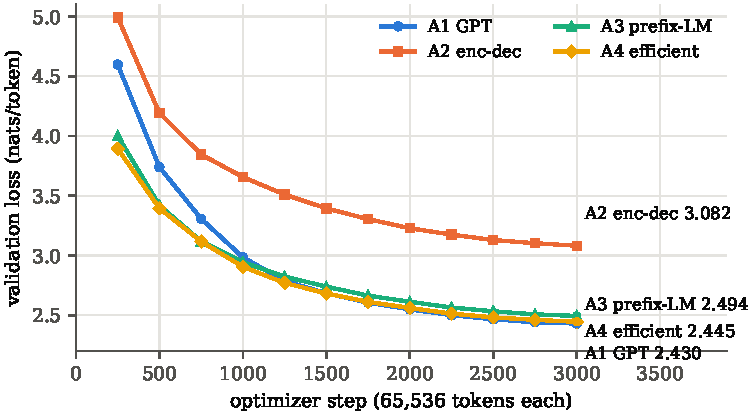
\includegraphics[width=0.82\linewidth]{figs/val_original.pdf}
\caption{Validation loss of the original runs (first corpus, old val). Final values are labelled.}
\label{fig:val-orig}\end{figure}

\begin{table}[H]\centering\small
\caption{Original Phase-1 runs (old val; dev metrics on the first dev set).}\label{tab:orig}
\begin{tabular}{lrrrrrrrr}\toprule
Model & Params & Non-emb. & Val loss & Val ppl & BERTScore & ROUGE-L & BLEU-4 & GPU-h\\\midrule
\tabinput{tables/original.tex}
\bottomrule\end{tabular}\end{table}

\subsection{Cleaned corpus}\label{sec:res-clean}
\autoref{tab:funnel} counts every document of the four files by outcome and \autoref{fig:reasons} ranks the
reasons.  In total \totdocsread{} documents were read; \totexactdup{} were exact duplicates,
\totneardup{} near duplicates (\nearduppairs{} verified pairs), \totstutter{} were dropped for heavy OCR
stutter and \totstutterrepaired{} were repaired and kept (\totstutterwords{} words removed).

\begin{table}[H]\centering\small
\caption{Documents per source by outcome of cleaning (before budget selection).}\label{tab:funnel}
\setlength{\tabcolsep}{4pt}
\begin{tabular}{lrrrrrrrr}\toprule
Source & Read & U+FFFD & Stutter & Too short & Few letters & Exact dup. & Near dup. & Available\\\midrule
\tabinput{tables/clean_funnel.tex}
\bottomrule\end{tabular}\end{table}

\begin{figure}[H]\centering
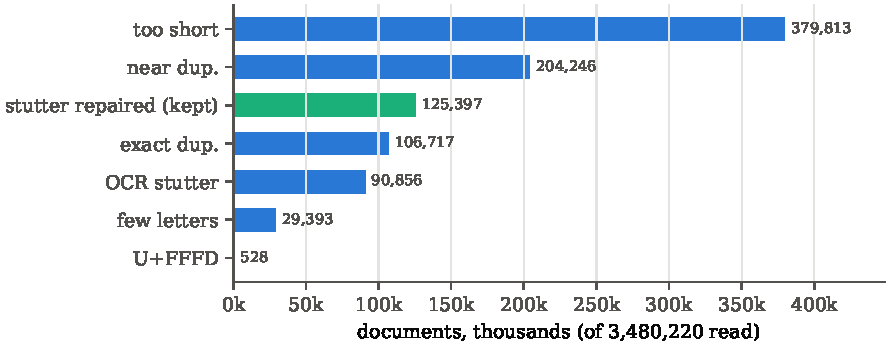
\includegraphics[width=0.78\linewidth]{figs/cleaning_reasons.pdf}
\caption{Documents removed by each rule (blue) and documents repaired by the stutter rule and kept (green).}
\label{fig:reasons}\end{figure}

\begin{table}[H]\centering\small
\caption{Budget selection and split. Target = token share by mixing ratio after redistribution (M6).}\label{tab:clean-select}
\begin{tabular}{lrrrrrr}\toprule
Source & Tokens/word & Target & Train tokens & Train docs & Val docs & Val dropped (leak)\\\midrule
\tabinput{tables/clean_selection.tex}
\bottomrule\end{tabular}\end{table}

\begin{figure}[H]\centering
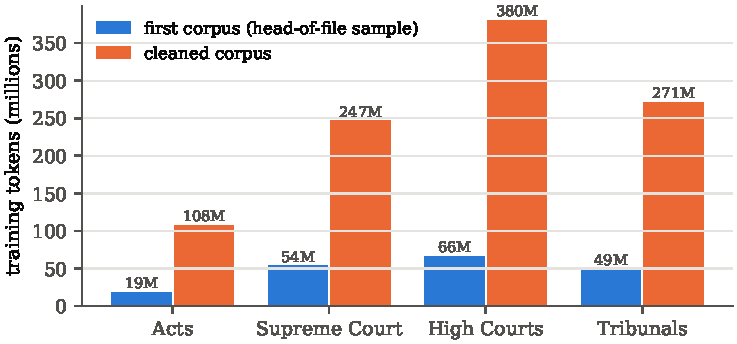
\includegraphics[width=0.8\linewidth]{figs/tokens_per_source.pdf}
\caption{Training tokens per source in the first and the cleaned corpus.}
\label{fig:tokens}\end{figure}

\subsubsection*{Audit of the cleaned corpus (M10)}
\autoref{tab:audit-ba} reruns the audit of \autoref{sec:audit} (\code{scripts/11\_audit\_corpus.py}) on both
corpora.  The cleaned corpus is 4.7 times larger, so rates are given next to counts.  Reading every record
(M7) also brought in text the first corpus never reached: \tribdeva{} Tribunal documents
(\tribdevapct\% of the source) contain Devanagari and \tribnonascii{} are more than 20\% non-ASCII, and
many High Court and Tribunal documents carry URLs.  These were not targeted by any cleaning rule.

\begin{table}[H]\centering\small
\caption{Audit before and after cleaning (counts, share of training documents).}\label{tab:audit-ba}
\begin{tabular}{lrr}\toprule
Check & First corpus & Cleaned corpus\\\midrule
\tabinput{tables/audit.tex}
\bottomrule\end{tabular}\end{table}

\subsection{Throughput}\label{sec:res-tput}
\begin{figure}[H]\centering
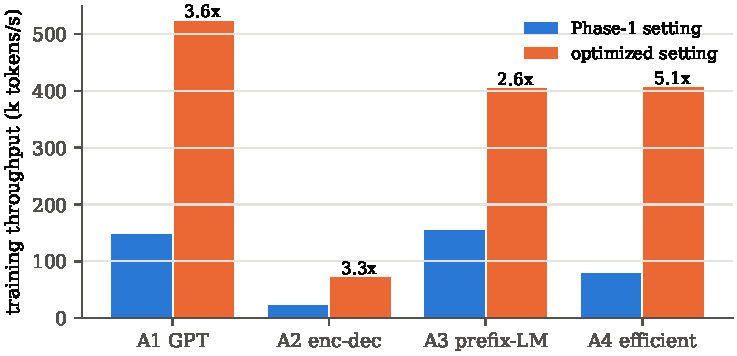
\includegraphics[width=0.8\linewidth]{figs/throughput.pdf}
\caption{Training throughput before and after the changes of \autoref{sec:throughput}. Benchmarks of 40--60
steps on the H200 while the corpus build was using the CPUs, so absolute numbers are lower than in an idle
machine; the ratios are the point.}
\label{fig:tput}\end{figure}

\begin{table}[H]\centering\small
\caption{Throughput benchmarks (tokens/s).}\label{tab:tput}
\begin{tabularx}{\linewidth}{lXr}\toprule
Model & Settings measured & Speed-up\\\midrule
\tabinput{tables/throughput.tex}
\bottomrule\end{tabularx}\end{table}

\subsection{Retraining}\label{sec:res-retrain}
\begin{figure}[H]\centering
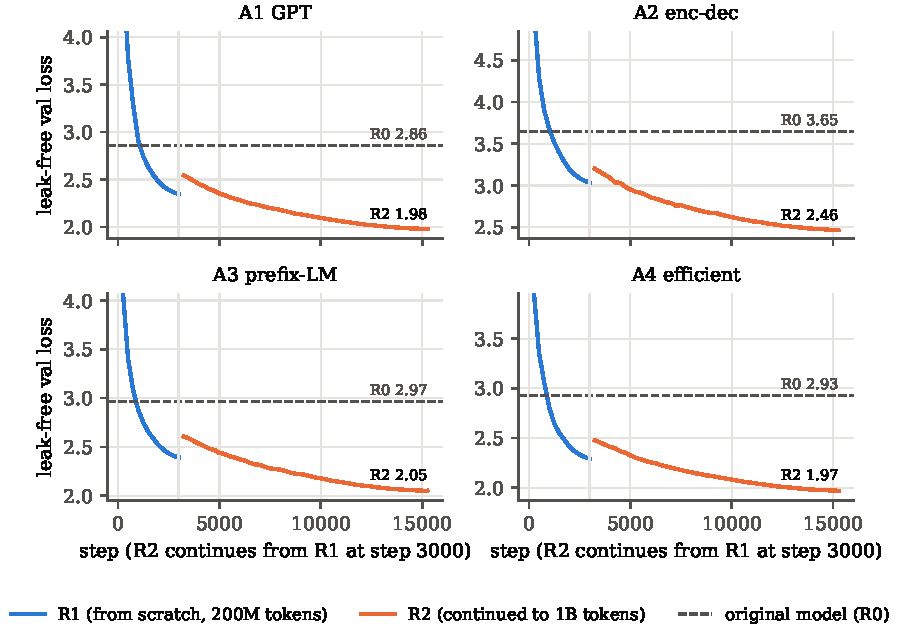
\includegraphics[width=0.92\linewidth]{figs/val_retrain.pdf}
\caption{Leak-free validation loss of R1 (steps 0--3{,}000) and R2 (continued from R1; the restarted
warm-up shows as the jump at step 3{,}000). The dashed line is the original model (R0) on the same set.}
\label{fig:retrain}\end{figure}

\begin{table}[H]\centering\small
\caption{Retraining runs. Throughput is the median over logged steps with two runs sharing the GPU.}\label{tab:compute}
\begin{tabular}{llrrrrr}\toprule
Model & Run & Steps & Tokens & Median tok/s & GPU-h & Peak alloc. (GB)\\\midrule
\tabinput{tables/compute.tex}
\bottomrule\end{tabular}\end{table}

\subsection{Evaluation on the three validation sets}\label{sec:res-eval}
\begin{figure}[H]\centering
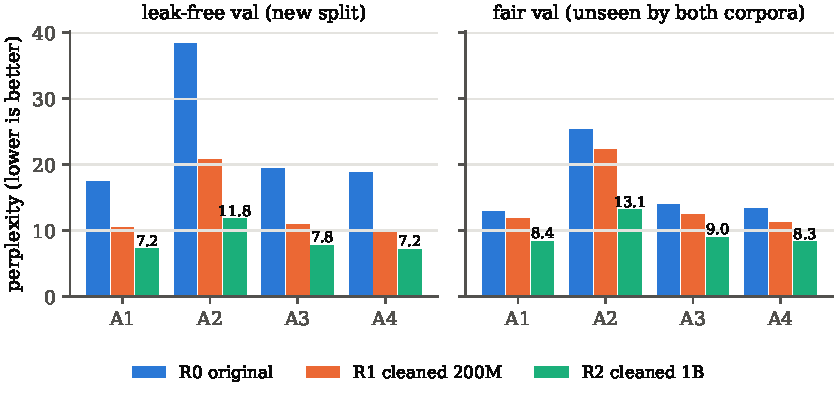
\includegraphics[width=0.92\linewidth]{figs/ppl_sets.pdf}
\caption{Perplexity of R0, R1 and R2 on the leak-free and the fair validation sets (R2 values labelled;
all values in \autoref{tab:results}).}
\label{fig:ppl}\end{figure}

\begin{table}[H]\centering\small
\caption{Perplexity on the three validation sets and generation metrics on the cleaned dev prompts (200
prompts from leak-free validation documents; R0 regenerated on the same prompts).}\label{tab:results}
\begin{tabular}{llrrrrrr}\toprule
& & \multicolumn{3}{c}{Perplexity} & \multicolumn{3}{c}{Dev generation}\\\cmidrule(lr){3-5}\cmidrule(lr){6-8}
Model & Run & Old val & Leak-free & Fair & BERTScore & ROUGE-L & BLEU-4\\\midrule
\tabinput{tables/results.tex}
\bottomrule\end{tabular}\end{table}

\begin{figure}[H]\centering
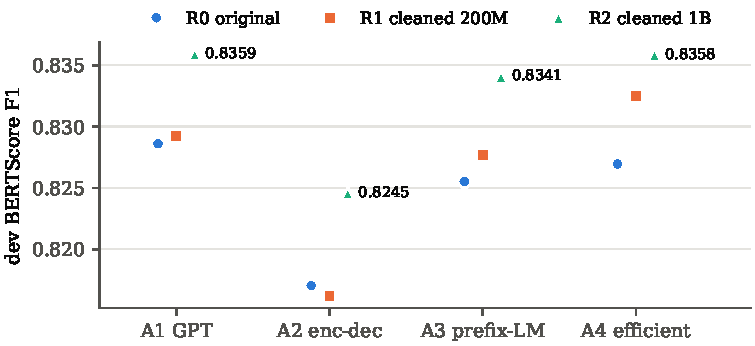
\includegraphics[width=0.8\linewidth]{figs/bertscore.pdf}
\caption{Dev BERTScore F1 on the cleaned dev prompts (R2 values labelled).}
\label{fig:bert}\end{figure}

On the old validation set, which favours the original models, A4~R1 scores a perplexity of 10.18 against
11.53 for the original A4 (\code{scripts/09\_eval\_val.py}).

\subsection{Test-set contamination}\label{sec:res-contam}
With the 13-gram test of M10 (a document counts if more than half of its sampled 13-grams occur in the
reference text):
\begin{itemize}
  \item \contamPone{} of the 1{,}000 Phase-1 test prompts and \contamPtwo{} of the 35 Phase-2 test documents
  overlap the training text (cleaned training split plus the first corpus) by more than 50\%.
  \item Against each corpus alone: Phase-2 test documents with $>$90\% overlap, 5 of 35 for the first corpus
  and 25 of 35 for the cleaned corpus; Phase-2 training documents, 8 of 70 and 50 of 70.
\end{itemize}
The test documents are part of the official training files, so reading every record (M7) includes them.
Nothing was removed; this is reported so that later phases can be interpreted with it in mind.

\subsection{Use as a starting point for later phases}\label{sec:res-transfer}
The Phase-1 checkpoints were reused as backbones.  Phase~2 (legal NER, A4 + LoRMA, mean macro-F1 over three
dev splits): original 0.488, R1 0.479, R2 0.467.  Phase~3 (rhetorical roles, A4 + LoRMA, out-of-fold
macro-F1 over 90 documents): original 0.427, R2 0.455.

% =====================================================================
\section{Analysis}\label{sec:analysis}
\authorbox{analysis of the results}{The course rules (§2, item 9) do not allow LLM-written result analysis.
Questions the course asks the report to answer (§7.4, §20.1), with the evidence above:
\begin{itemize}
  \item Which architecture works best under the same budget, and why (\autoref{fig:val-orig} and \autoref{tab:orig})?
  \item How did data quality and data quantity each affect the models (R0 vs R1 vs R2, \autoref{tab:results})?
  \item How much did the leaky validation split change the conclusions one would draw (old vs fair val)?
  \item What did the throughput changes cost or save (\autoref{tab:tput} and \autoref{tab:compute})?
  \item Why might a lower perplexity not transfer to every downstream task (\autoref{sec:res-transfer})?
  \item What failed, and why (e.g.\ A2's encoder output, \code{torch.compile} on A2, four concurrent runs)?
\end{itemize}}

\section{Limitations and next steps}
Facts that limit the conclusions (the interpretation is the author's):
\begin{itemize}
  \item One seed per run; no confidence intervals on perplexity or BERTScore.
  \item Decoding was not tuned on the new models (one setting, \autoref{sec:setup}).
  \item No Phase-1 compression experiment was run on the cleaned models (a distillation config exists:
  \code{configs/distill\_efficient\_small.yaml}).
  \item The cleaning thresholds (\autoref{tab:cleancfg}) were set once, not ablated individually; R1 measures
  all of M1--M7 together.
  \item Downstream test documents occur in the cleaned training text (\autoref{sec:res-contam}).
  \item Throughput benchmarks ran on a shared machine under CPU load.
  \item The cleaned corpus contains Hindi/Devanagari Tribunal documents and URLs (\autoref{tab:audit-ba}),
  which no rule filtered; their share and effect were not measured separately.
  \item Template headers remain: \autoref{tab:audit-ba} still finds documents sharing their first 300
  characters (different bodies, so not near duplicates).
\end{itemize}
\authorbox{what you would do next}{With more time or compute: \ldots}

\section{Conclusions}
\authorbox{conclusions}{Summarise what you conclude from the experiments, in your own words.}

\section{Reproducibility}
Code: \code{capstone\_llm/} (Phase~1).
\authorbox{repository link}{GitHub: \url{https://github.com/...}}
\noindent{\small\begin{tabularx}{\linewidth}{l>{\raggedright\arraybackslash}X}
First pipeline & \code{bash run\_all.sh}\\
Cleaned corpus & \code{python scripts/01\_prepare\_data.py --config configs/base.yaml configs/clean.yaml}\\
Tokenize & \code{python scripts/03\_tokenize.py --config configs/base.yaml configs/clean.yaml}\\
R1 + R2, all models & \code{bash run\_clean.sh}\\
R0 on another val set & \code{python scripts/09\_eval\_val.py --val data\_clean/tokens/val.bin --ckpt ...}\\
Fair val & \code{python scripts/10\_fair\_val.py}\\
Corpus audit & \code{python scripts/11\_audit\_corpus.py data\_clean/corpus}\\
Figures and tables & \code{python p1/report/make\_figures.py}\\
\end{tabularx}}

\section*{LLM declaration}
\authorbox{LLM declaration (mandatory)}{Fill in the course questionnaire.  Describe honestly which parts used
an LLM assistant (for example code for the cleaning pipeline, scripts, figures and this report's
methods/results text) and which parts are your own (design decisions, hyperparameters, analysis, conclusions).}

\begin{thebibliography}{99}\small
\bibitem{ainslie2023gqa} J.~Ainslie et al. GQA: Training generalized multi-query transformer models from multi-head checkpoints. EMNLP 2023.
\bibitem{beltagy2020longformer} I.~Beltagy, M.~Peters, A.~Cohan. Longformer: The long-document transformer. arXiv:2004.05150, 2020.
\bibitem{broder1997resemblance} A.~Broder. On the resemblance and containment of documents. Compression and Complexity of Sequences, 1997.
\bibitem{hoffmann2022chinchilla} J.~Hoffmann et al. Training compute-optimal large language models. NeurIPS 2022.
\bibitem{holtzman2020curious} A.~Holtzman et al. The curious case of neural text degeneration. ICLR 2020.
\bibitem{keskar2019ctrl} N.~Keskar et al. CTRL: A conditional transformer language model for controllable generation. arXiv:1909.05858, 2019.
\bibitem{lee2022dedup} K.~Lee et al. Deduplicating training data makes language models better. ACL 2022.
\bibitem{leskovec2014mmds} J.~Leskovec, A.~Rajaraman, J.~Ullman. Mining of Massive Datasets, ch.~3. Cambridge University Press, 2014.
\bibitem{lin2004rouge} C.-Y.~Lin. ROUGE: A package for automatic evaluation of summaries. ACL Workshop 2004.
\bibitem{loshchilov2019adamw} I.~Loshchilov, F.~Hutter. Decoupled weight decay regularization. ICLR 2019.
\bibitem{papineni2002bleu} K.~Papineni et al. BLEU: a method for automatic evaluation of machine translation. ACL 2002.
\bibitem{press2022alibi} O.~Press, N.~Smith, M.~Lewis. Train short, test long: Attention with linear biases enables input length extrapolation. ICLR 2022.
\bibitem{radford2019gpt2} A.~Radford et al. Language models are unsupervised multitask learners. OpenAI, 2019.
\bibitem{raffel2020t5} C.~Raffel et al. Exploring the limits of transfer learning with a unified text-to-text transformer. JMLR 2020.
\bibitem{sennrich2016bpe} R.~Sennrich, B.~Haddow, A.~Birch. Neural machine translation of rare words with subword units. ACL 2016.
\bibitem{shazeer2020glu} N.~Shazeer. GLU variants improve transformer. arXiv:2002.05202, 2020.
\bibitem{su2021roformer} J.~Su et al. RoFormer: Enhanced transformer with rotary position embedding. arXiv:2104.09864, 2021.
\bibitem{vaswani2017attention} A.~Vaswani et al. Attention is all you need. NeurIPS 2017.
\bibitem{zhang2019rmsnorm} B.~Zhang, R.~Sennrich. Root mean square layer normalization. NeurIPS 2019.
\bibitem{zhang2020bertscore} T.~Zhang et al. BERTScore: Evaluating text generation with BERT. ICLR 2020.
\end{thebibliography}
\end{document}
